\documentclass[12pt]{article}
\usepackage{algo,fullpage,url,amssymb,epsfig,color,xspace,tikz,amsmath}
\usepackage[pdftitle={CS 240 Assignment 2},
pdfsubject={University of Waterloo, CS 240, Fall 2016},
pdfauthor={Arne Storjohann}]{hyperref}
\usepackage{graphicx}
\renewcommand{\thesubsection}{Problem \arabic{subsection}}
\begin{document}
\vspace*{-2cm}
\begin{center}
{\Large\bf University of Waterloo}\\
\vspace{3mm}
{\Large\bf CS240 - Fall 2016}\\
\vspace{2mm}
{\Large\bf Assignment 2}\\
\vspace{3mm}
\textbf{Due Date: Wednesday October 5 at 5pm}
\end{center}

\definecolor{care}{rgb}{0,0,0}
\def\question#1{\item[\bf #1.]}
\def\part#1{\item[\bf #1)]}
\newcommand{\pc}[1]{\mbox{\textbf{#1}}} % pseudocode

Please read
\url{http://www.student.cs.uwaterloo.ca/~cs240/f16/guidelines.pdf}
for guidelines on submission.  All problems are written problems;
submit your solutions electronically as a PDF with file name {\tt
a02wp.pdf} using MarkUs. We will also accept individual question
files named {\tt a02q1w.pdf}, {\tt a02q2w.pdf}, ... ,{\tt a02q5w.pdf}
if you wish to submit questions as you complete them.  

There are 65 possible marks available.  The assignment will be
marked out of 60.

%%%%%%%%%%%%%%%%%%%%%%%%%%%%%%%%%%%%%%%%%%%%%%%%%%%%%%%%%%%%%
\subsection{[5+5+5=15 marks]}
Consider a very keen teaching assistant.
As students arrive during office hour she assigns a priority number
to each student corresponding to their time of arrival and inserts the
pair (time, name) into a priority queue, implemented as a min-heap. The
next student is determined with a call to {\tt deleteMin}. The student
then has five minutes to ask as many questions as possible before being
re-inserted in the queue with the current time as priority.

Occasionally students leave before their turn comes up.  Describe how
to perform a delete key operation in a heap under each of the following
assumptions:
\begin{enumerate}
\part{a} The input for the delete operation is the student name only,
assumed to be unique.
\\\textbf{Solution:}
\\Because we do not know the time/priority of the student, we cannot directly apply the properties of minHeap to this question. Since we want to delete that student, we can swap him/her with the last student in the array. Then, doing a bubble-down operation to the initial last student in the array to reach his/her position in the queue. The first operation needs $O(n)$ to search the student's name in the queue for the worst case. The second operation needs $O*\log{n})$ (height of the heap) to put the initial last student to the correct position. So, this question requires $O(\log{n}) + O(n) \in O(n)$ steps.
\part{b} The input for the delete operation is the priority
value in the heap, again assumed to be unique.
\\\textbf{Solution:}
\\This question is similar to the previous. Even though we know the priority value of that student, it may still take us $O(n)$ to compare the priority value with those of other students' for the worst case. After finding him/her, swap with the last student. Then, using $O(\log{n})$ to do the bubble-down operation to get the initial last student to the correct position. Thus, totally $O(\log{n}) + O(n) \in O(n)$steps are required. 
\part{c} The input to the delete operation is the index
 of the entry in the array where the key resides.
\\\textbf{Solution:}
\\This question is straight-forward since we know the index of the student we want to find, it takes $O(1)$ to reach that student. Similarly, we do bubble-down swapping operations to put this student into the correct position. Thus, the worst case is the height of the heap, which is $O(\log{n}) \in o(n)$. 
\end{enumerate}
In each case the priority queue is implemented as a heap using an
array. After the delete operation the array should still be a heap.
For each implementation discuss the time complexity of the operation in
the worst case.  The running time of all of your methods should be $O(n)$, and
at least one of the methods should have running time $o(n)$.
%%%%%%%%%%%%%%%%%%%%%%%%%%%%%%%%%%%%%%%%%%%%%%%%%%%%%%%%%%%%%
\subsection{[10 marks]}
A sorting algorithm is said to sort \emph{in place} if only a constant
number of elements of the input are ever stored outside the array.
In class we showed that all comparison based sorting algorithms
require $\Omega(n \log n)$ comparisons to sort an array of length
$n$.  But suppose are given an array $A[0\ldots n-1]$ that contains a
permutation of the first $n$ non-negative integers.
Allowing non comparison
based algorithms, give an $O(n)$ in place algorithm to sort $A$.  Analyze the
the running time of your method.
{\em Note:} For simplicity we are assuming $A$ is filled with
integer keys.  Your algorithm must easily extend to work for an array
$A$ that is filled with (key,element) pairs, each integer key in the
range $0\ldots n-1$ occurring exactly once.
\\
\\\textbf{Solution:}
\\Sudo code for this question:
\\\textit{for int i = 0 to n-1, do:
\\if A[i].key != i;
\\swap(A[i], A[A[i].key]);
\\else
\\continue;}
\\
\\Since we know the index of each element, we can just arrange all elements to their right positions based on their key field. My idea is to go through the array from the first element, if the element is in its correct position, then jump to the next index. If not, swap the element with the one that should be in the current index. We repeat these procedures until the last index is checked. The algorithm is $O(n)$ because we go through each index from 0 to $n-1$, and for the worst case, all elements are not in correct positions. 
%%%%%%%%%%%%%%%%%%%%%%%%%%%%%%%%%%%%%%%%%%%%%%%%%%%%%%%%%%%%%
\subsection{[10 marks]}
You are given an unsorted array $A[0\ldots n-1]$ filled with
distinct integers. For a given $k$, $1\leq k\leq n$, describe an in-place
algorithm that rearranges the array so that $A[0\ldots k-1]$ contains
the $k$ smallest integers in increasing order.  If $k \in O(n/\lg n)$ 
your algorithm should have running time $O(n)$.  Analyze the running
time of your algorithm.
\\\textbf{Solution:}
\\Firstly, we need to find the $k^{th}$ largest element in this unsorted array. Thus, we can use $QuickSelect(A, k)$ to find the $k^{th}$ largest value, which takes $O(n)$ runtime. Secondly, let the $k^{th}$ value be $n$, we can use $partition(A, n)$ to put all elements which are equal or less than n to positions before $n$, which takes $O(n)$ runtime. Lastly, we can use mergesort algorithm to sort the array before $n$. And the last step takes $O(k\log{k})$ runtime.
\\
\\Thus, for the overall runtime, we have:
\\$O(n) + O(n) + O(k\log{k})$
\\
\\$\leq O(n) + O(n) + O(\frac{n}{\log{n}}\log{\frac{n}{\log{n}}})$ (given in the question)
\\
\\$= 2O(n) + O(\frac{n}{\log{n}}(\log{n} - \log{\log{n}})) $
\\
\\$=2O(n) + O(n - \frac{n\log{\log{n}}}{\log{n}})$
\\
\\$\leq 2O(n) + O(n)$
\\
\\$=3O(n)$
\\
\\$\in O(n)$
%%%%%%%%%%%%%%%%%%%%%%%%%%%%%%%%%%%%%%%%%%%%%%%%%%%%%%%%%%%%%
\subsection{[6+7+7=20 marks]}
\begin{center}
        
\includegraphics[scale=0.05]{chest.png} 
\mbox{~~~~~~~~~~~~~~~~~~~~~~}
        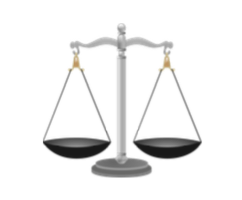
\includegraphics[scale=0.05]{balance.png}
\end{center}
You have found a treasure chest filled with $n$ coins, some of which
are genuine and some of which are counterfeit.  There is at least one
genuine coin and at least one counterfeit coin in the chest.
All genuine coins weigh the same and all counterfeit coins weigh the
same, but the counterfeit coins weigh less than the genuine coins.  
Your task is to separate the genuine coins from the counterfeit
coins.  To accomplish this you will compare the weight of pairs of
subsets of the coins using a balance scale.  The outcome of one weighing
will determine that each subset of coins weighs the same, or that one
or the other subset of coins weighs more.
\begin{itemize}
\part{a} [6 marks] Give a precise (not big-Omega) lower bound for
the number of weighings required in the worst case to determine which
coins are genuine and which are counterfeit.
\\\textbf{Solution:}
\\The precise lower bound for the number of weighings reequired in the worst case is $(n-1)$, since we need to do one-on-one comparisons for $(n-1)$ times. There are two scenarios in this case.
\\
\\\textit{Case 1:} For the comparisons between the first pair of coins, if there appears the difference between the two coins shown on the balance, we will easily know which one is genuine and which one is counterfeit. So in the subsequent one-on-one comparisons, it will be really easy to differ whether the coin is genuine or counterfeit by comparing either of the coins in the first comparison.
\\
\\\textit{Case 2:} If the first k coins are all counterfeit or genuine, where $1 < k < n-1$, we cannot distinguish whether they are all counterfeit or genuine. We just put them together beside. However, there is a precondition in this question is that there is at least one counterfeit and one genuine coin, that means there will definitely be one pair with different coins. For example, if the first four coins we compare are counterfeit (we do not know) in a 6-coins set, if the fifth coin is genuine, we can know that the first four coins are counterfeit. This case still costs $(n-1)$ runtime.
\part{b} [7 marks] Describe an algorithm called \texttt{FindGenuine}
to determine the genuine coins when \mbox{n\,=\,4}. Use the names
C1, C2, C3, C4 for the four coins, and the function
\[ CompareWeight\left( \{ first\_subset; second\_subset\} \right), \]
which returns either ``first weighs more'', ``second weighs more'', 
or ``both weigh the same''.
Your function should return the set of genuine coins.

Give an exact worst-case analysis of the number of weighings required
by your algorithm.  For full marks, this should match exactly the
lower bound from Part (a) when $n = 4$.
\\\textbf{Solution:}
\\\textit{Sudo code:}
\\\textit{count = 0;
\\for int i = 1 to 3, do
\\CompareWeight($C_i$, $C_{i+1}$)
\\if "first weighs more", then
\\Insert(genuine, $C_i$)
\\count++
\\if "second weighs more", then
\\Insert(genuine, $C_{i+1}$)
\\count++
\\else
\\if count != 0, then 
\\Insert(genuine, $C_{i+1}$)
\\else
\\Insert(temp, $C_{i+1}$)
\\done
\\if temp == empty or (temp[0] < genuine[0])
\\return genuine
\\else
\\return genuine + temp
\\}
\\The count variable checks if the first k consecutive coins are the same type (i.e., count = 0), then store them in a temp array. If count != 0, then it means the coin we compared to is the genuine coin, which can directly be put into the genuine set. The return genuine set is the original genuine set and the temp set if the coins stored in the temp set are genuine coins. 
\part{c} {[7 marks]} Describe an algorithm to determine the genuine
coins, for any $n$. Use the names C1, C2, ... , Cn and
the $CompareWeight$ subroutine from Part (b). Show that your algorithm is
asymptotically optimal, meaning that the big-O cost should match
the lower bound from Part (a).
\\\textbf{Solution:}
\\\textit{Sudo code:}
\\\textit{count = 0;
\\for int i = 1 to n, do
\\CompareWeight($C_i$, $C_{i+1}$)
\\if "first weighs more", then
\\Insert(genuine, $C_i$)
\\count++
\\if "second weighs more", then
\\Insert(genuine, $C_{i+1}$)
\\count++
\\else
\\if count != 0, then 
\\Insert(genuine, $C_{i+1}$)
\\else
\\Insert(temp, $C_{i+1}$)
\\done
\\if temp == empty or (temp[0] < genuine[0])
\\return genuine
\\else
\\return genuine + temp
}
\\
\\It is the same logic as part(b), just change 4 to n. 
\end{itemize}
%%%%%%%%%%%%%%%%%%%%%%%%%%%%%%%%%%%%%%%%%%%%%%%%%%%%%%%%%%%%%
\subsection{[4+6=10 marks]}
A \emph{deterministic} algorithm is one whose execution depends
only on the input. By contrast, the execution of a \emph{randomized}
algorithm depends also on some randomly-chosen numbers. A \emph{Las
Vegas} randomized algorithm always produces the correct answer, but
has a running time which depends on the random numbers chosen
(randomized quick-select and quick-sort are of this type). Informally,
such algorithms are always correct, and probably fast. A \emph{Monte
Carlo} randomized algorithm has running time independent of the
random numbers chosen, but may produce an incorrect answer. Informally,
such algorithms are always fast, and probably correct.

Given an array A of length n, an element x is said to be \emph{dominant}
in A if x occurs at least $\lfloor n/2 \rfloor + 1$ times in A.
That is, copies of x occupy more than half of the array.
\begin{itemize}
\part{a} [4 marks] Given an array A that contains a dominant element,
describe an in-place Monte Carlo randomized algorithm to find the dominant
element. Show that your algorithm has worst-case running time $O(1)$
and returns the correct answer with probability at least 1/2.
\\\textbf{Solution:}
\\Randomly generate an integer k, where $0 \leq k \leq n-1$, and return A[k]. Because the question said that there is a dominant element in A, which means we have more than 50\% chance to luckily pick up an element that is dominant. Thus, the worst-case running time is $O(1)$ in this scenario. 
\part{b} [6 marks] Given an array A that contains a dominant element,
describe an in-place Las Vegas randomized algorithm to find the dominant
element. Show that your algorithm always returns the correct answer,
and has expected-case running time $O(n)$.
\\\textbf{Solution:}
\\\textit{Sudo code:}
\\\textit{int count = 0, dominant, i,
\\for i = 0 to n-1, do
\\if (count == 0), then
\\dominant = A[i];
\\if (A[i] == dominant), then
\\count++;
\\else
\\count--;
\\done
}
\\
\\Based on the definition of dominant element, the number of the dominant element is always larger than the number of non-dominant elements, which means[ $d$ (\# of dominant element) $- nond$ (\# of non-dominant elements) $\geq 1$]. Use this property, I create a \textit{count} variable to check which element is dominant so far when going through the entire array $A$. If $count == 0$, change the dominant to the next element. Otherwise, if the next element is equal to the dominant element so far, count plus one. If not, count minus one, and \textit{dominant} stays the same until \textit{count} goes to zero again. This algorithm is always correct in this question, and takes $O(n)$ runtime. 
\end{itemize}
\end{document}
